\documentclass[handout]{beamer}
%\documentclass [serif,mathserif,professionalfont]{beamer}
%\usepackage {pxfonts}
%\usepackage {eulervm}
%\usepackage{mathpazo}
%\logo{\includegraphics[height=1.2cm]{fsulogo.png}}

\usepackage{tikz}
\usepackage{graphicx}
\usepackage{multimedia}
\usepackage{subfig,fixltx2e,url}
\usepackage[latin1]{inputenc}
%\usetheme{Warsaw}
\usecolortheme{lily}
\setbeamercovered{transparent}
%\useoutertheme[subsection=false]{smoothbars}

\setbeamertemplate{sidebar right}{}
\setbeamertemplate{footline}{%
\hfill\usebeamertemplate***{navigation symbols}
\hspace{1cm}\insertframenumber{}/\inserttotalframenumber}

\title[ \insertdate]{Diversity in Fashion Recommendation Using Semantic Parsing}

\author{Sagar Verma\inst{1}, Sukhad Anand\inst{1}, Chetan Arora\inst{1}, Atul Rai\inst{2}}
\institute[IIIT Delhi and Staqu Technologies] % (optional, but mostly needed)
{
  \inst{1}%
  Department of Computer Science and Engineering\\
  Indraprastha Institute of Information Technology, Delhi.
  \and
  \inst{2}%
  Staqu Technologies}
% - Use the \inst command only if there are several affiliations.
% - Keep it simple, no one is interested in your street address.

\date{ICIP, 2018}
% - Either use conference name or its abbreviation.
% - Not really informative to the audience, more for people (including

\begin{document}

\begin{frame}
\titlepage
\end{frame}

\section{Recommendation based on contextual similarity}

\begin{frame}{Problem Statement}
\begin{center}
{\Large Recommendation based on contextual similarity}\\
\vspace{.5cm}
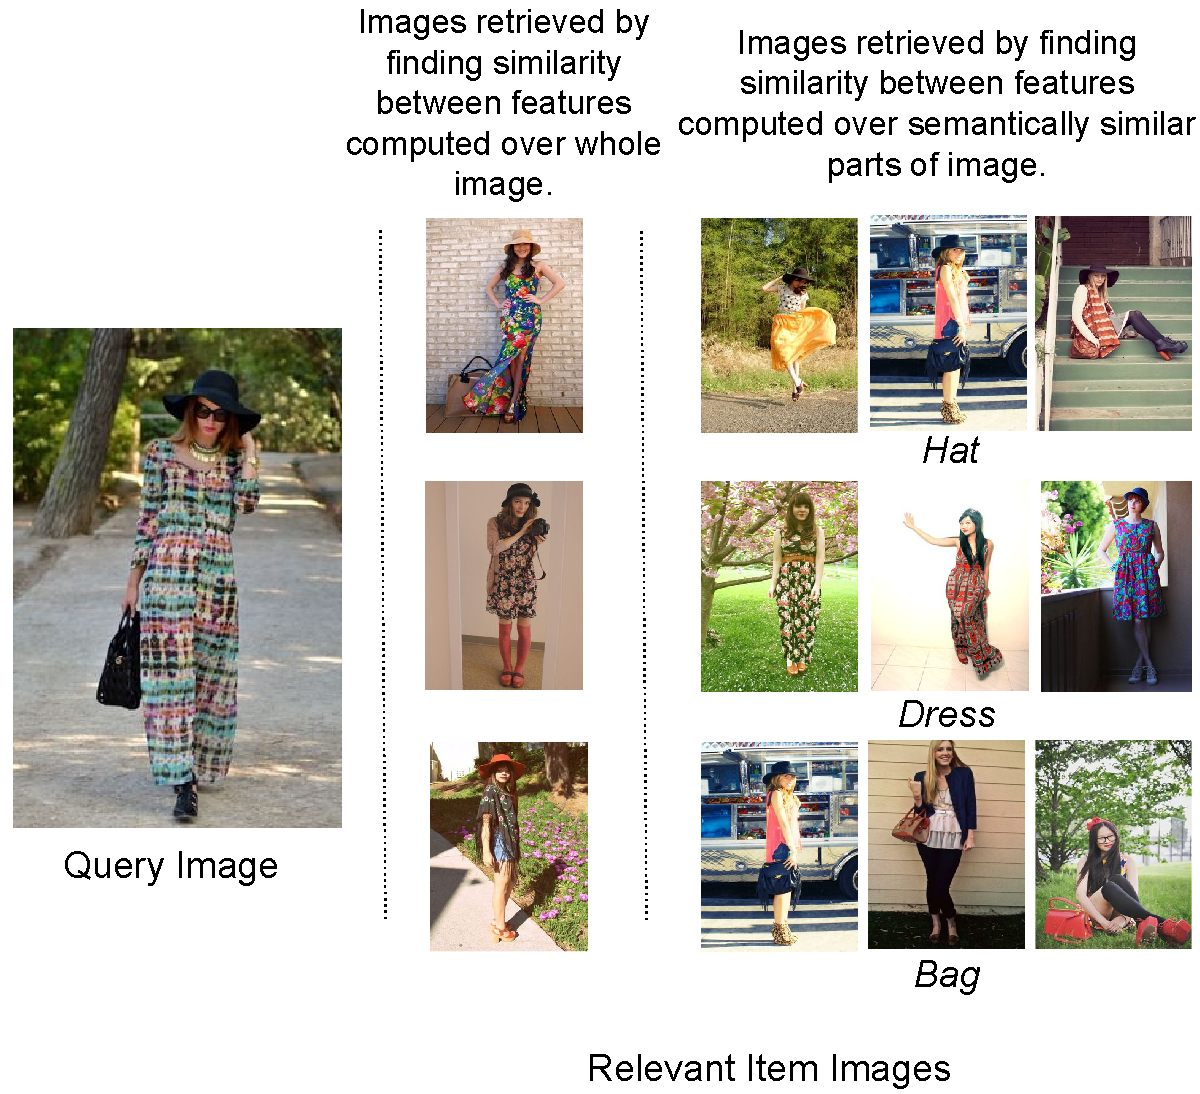
\includegraphics[width=0.8\linewidth, height=7cm]{images/teaser_staqu_texture}
\end{center}
\end{frame}


\begin{frame}{Contributions}
  \begin{enumerate}
    \item Our method recommends similar images based on different parts of a query image.

    \item To identify different parts we use attention and weakly labeled data.

    \item Instead of features from standard pre-trained neural networks, we suggest using texture-based features.

    \item We evaluate our method on item recognition task, consumer-to-shop retrieval and in-shop retrieval tasks.
  \end{enumerate}
\end{frame}

\begin{frame}{Related Work}
  \begin{itemize}
    \item Cloth parsing,
    \item Clothing attribute recognition,
    \item Detecting fashion style, and
    \item Cross-domain image retrieval using Siamese network and Triplet network.
  \end{itemize}
\end{frame}

\begin{frame}{Proposed Architecture}
  \vspace{-1cm}
    \begin{center}
      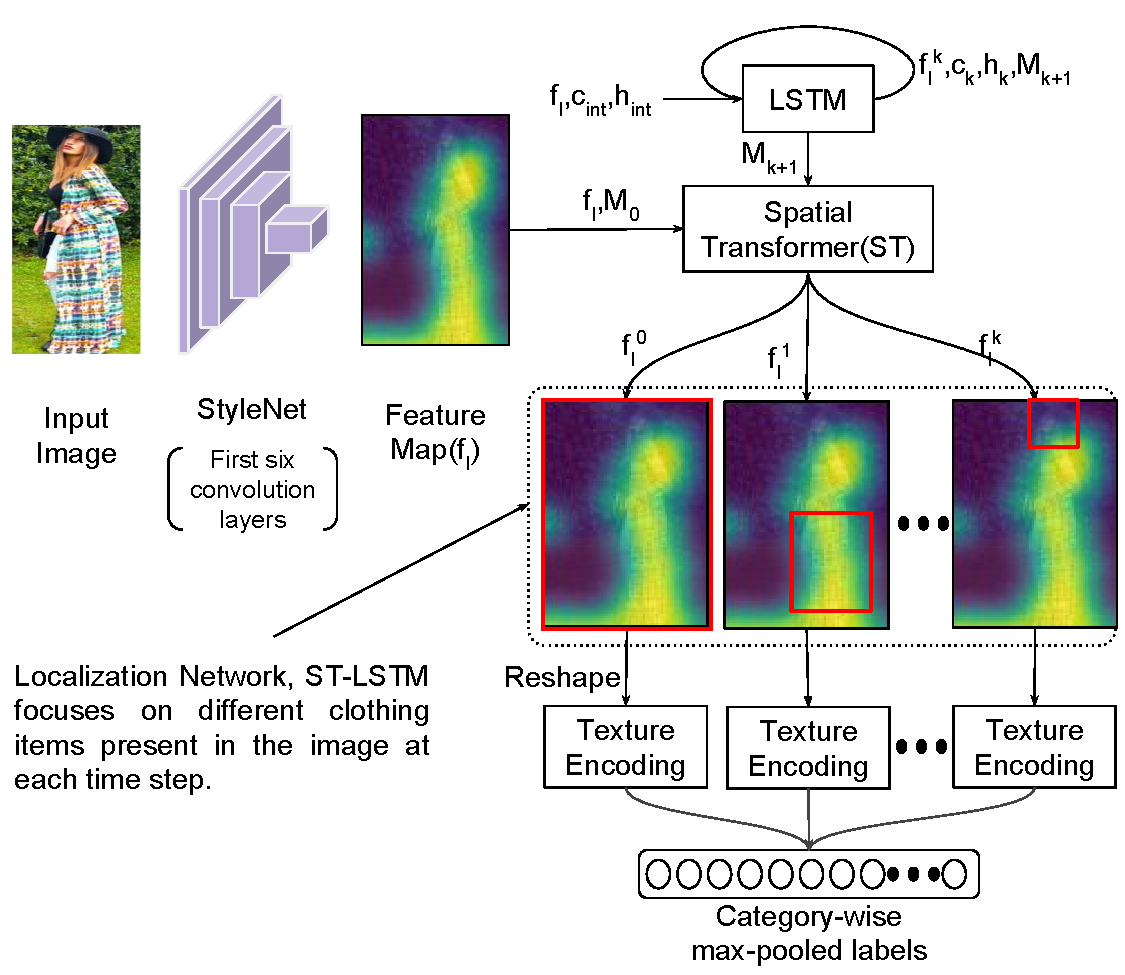
\includegraphics[width=0.8\linewidth, height=7cm]{images/staqu_st_ten_arch}
    \end{center}
\end{frame}

\begin{frame}{CNN for Global Image Features}
  \vspace{-1cm}
    \begin{center}
      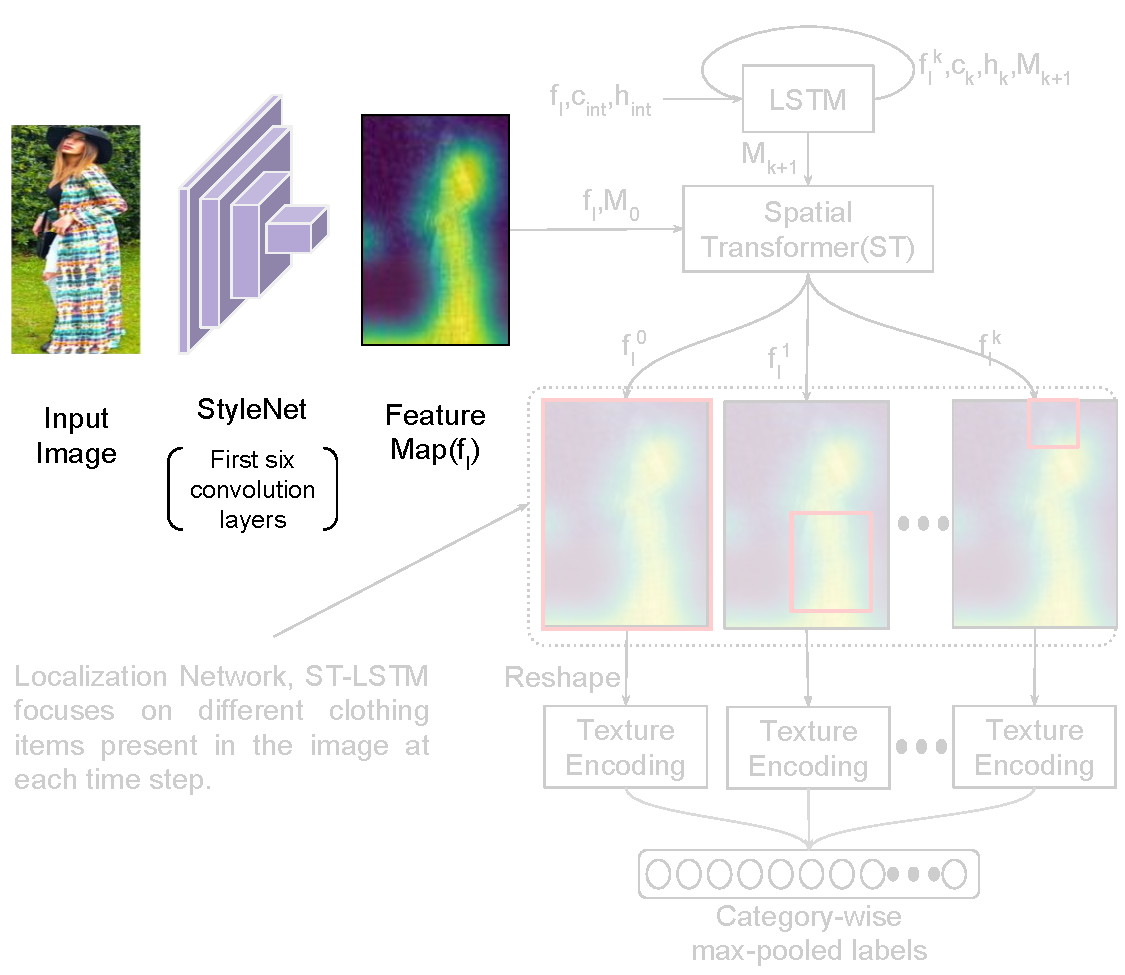
\includegraphics[width=0.8\linewidth, height=7cm]{images/staqu_st_ten_arch_cnn}
    \end{center}
\end{frame}

\begin{frame}{Visual Attention Module}
  \vspace{-1cm}
    \begin{center}
      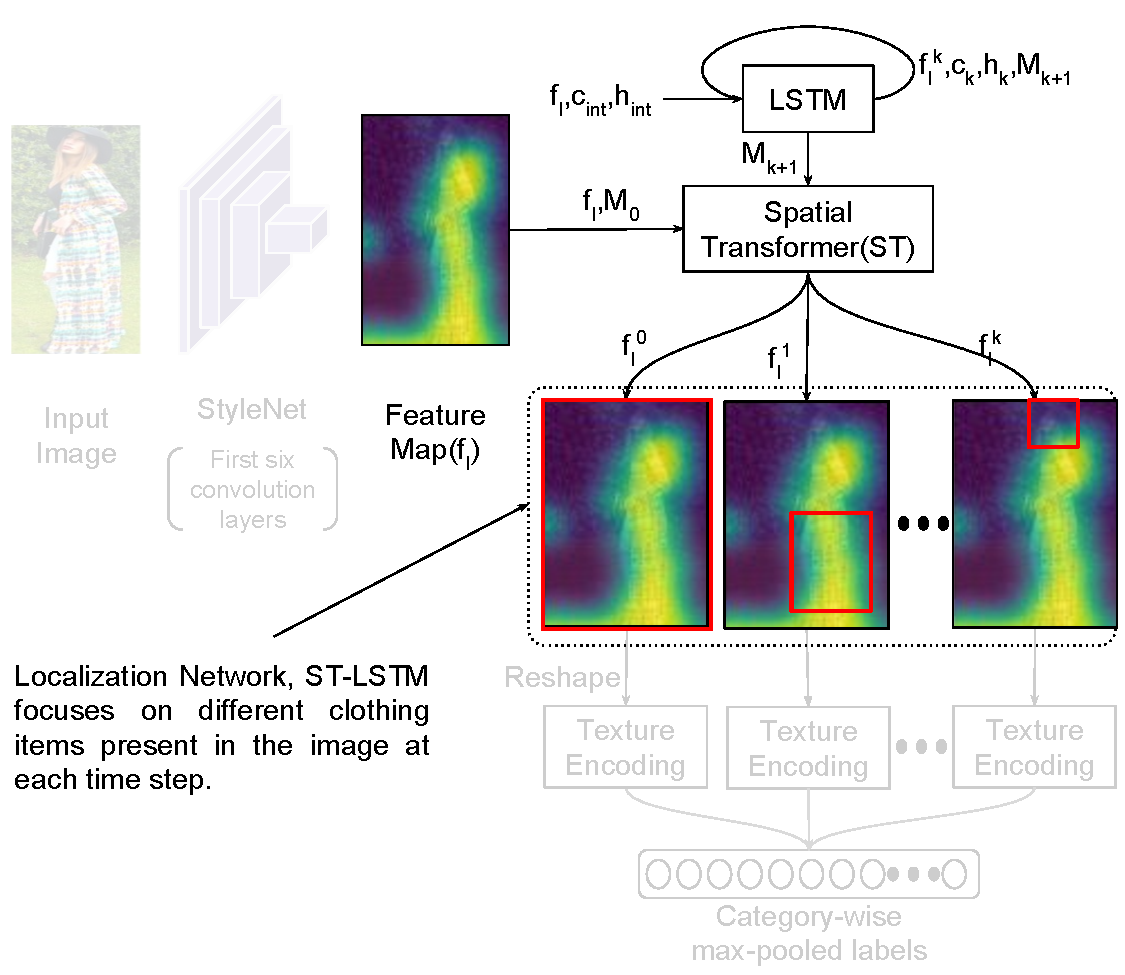
\includegraphics[width=0.8\linewidth, height=7cm]{images/staqu_st_ten_arch_attn}
    \end{center}
\end{frame}

\begin{frame}{Texture Encoding Layer}
\vspace{-1cm}
  \begin{center}
    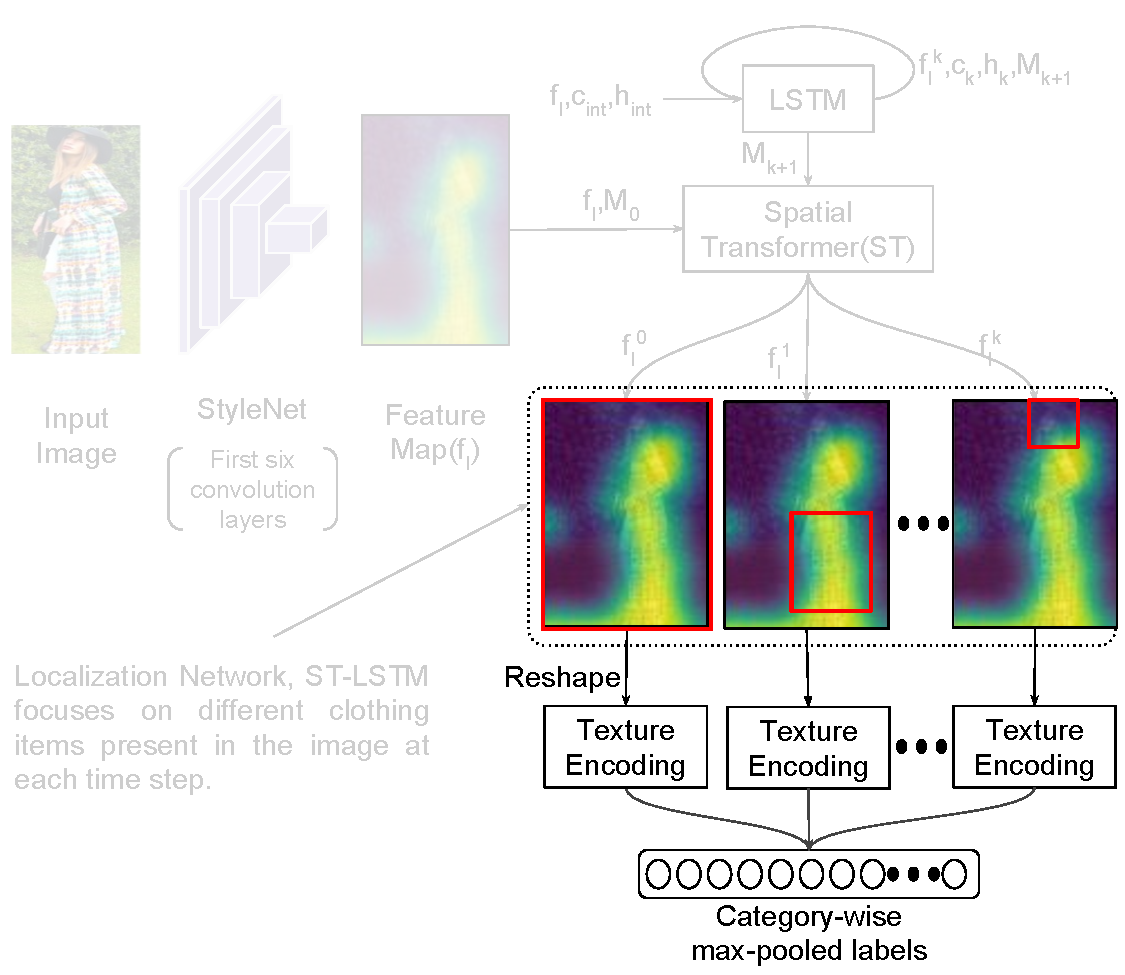
\includegraphics[width=0.8\linewidth, height=7cm]{images/staqu_st_ten_arch_text}
  \end{center}
\end{frame}

\begin{frame}{Multi-label classification loss}
      \begin{equation}
        \mathcal{L}_{cls} = \frac{1}{N} \sum^N_{i=1}\sum^C_{c=1}(p^c_i-\hat{p}^c_i)^2
      \end{equation}
      where, $N$ is training sample, $C$ is total number of classes, $\hat{p}_i$ is ground truth label vector of sample $i$ and $p_i$ is predicted label vector of sample $i$.
\end{frame}

\begin{frame}{Diversity loss}
  Diversity loss is the correlation between adjacent attention maps,
  \begin{equation}
    \mathcal{L}_{div} = \frac{1}{K-1} \sum^K_{k=2}\sum^{HxW}_{i=1} l_{k-1,i}.l_{k,i}
  \end{equation}
  where, $K$ is the total steps of recurrent attention, $HxW$ is the height and width of attention maps, $l_{k}$ is the $k^{th}$ attention map.
\end{frame}

\begin{frame}{Localisation loss}
  Localization loss, $\mathcal{L}_{loc}$ from \cite{WangSTLSTMICCV2017} is used to remove redundant locations and force localization network to look at small clothing parts.
\end{frame}

\begin{frame}{Combined Loss}
  \begin{equation}
    \mathcal{L} = \mathcal{L}_{cls} + \lambda_1\mathcal{L}_{div} + \lambda_2\mathcal{L}_{loc}
  \end{equation}
  where $\lambda_1$ and $\lambda_2$ are multiplicative factors. We use $0.01$ for all our experiments.
\end{frame}

\begin{frame}{Datasets}
  \begin{itemize}
    \item \textbf{Fashion144K \cite{SimoSerraCVPR2016}}
    \begin{itemize}
      \item 90,000 images with multilabel annotation.
      \item 128 classes.
      \item Image resolution is $384x256$.
    \end{itemize}

    \item \textbf{Fashion550K \cite{InoueICCVW2017}}
      \begin{itemize}
        \item 66 classes.
      \end{itemize}

    \item \textbf{DeepFashion \cite{LiuCVPR2016}}
      \begin{itemize}
        \item 800,000 images
        \item Similarity pairs is available for consumer-to-shop and in-shop retrieval tasks
      \end{itemize}
  \end{itemize}
\end{frame}

\begin{frame}{Experiments}
  \begin{itemize}
    \item Model is trained on Fashion144K \cite{SimoSerraCVPR2016} dataset with 59 item labels, color labels were excluded.
    \item Evaluated item recognition task on Fashion144K \cite{SimoSerraCVPR2016} and Fashion550K \cite{InoueICCVW2017} dataset.
    \item Consumer-to-shop and in-shop retrieval tasks are evaluated on DeepFashion \cite{LiuCVPR2016} dataset.
  \end{itemize}
\end{frame}

\begin{frame}{Results}
  \begin{table}
    \centering
    \begin{tabular}{ l c c c c}
       \hline
      Dataset & \multicolumn{2}{c}{Fashion144k \cite{SimoSerraCVPR2016}} & \multicolumn{2}{c}{Fashion550k \cite{InoueICCVW2017}} \\
      Model & \textit{AP}\textsubscript{all} & \textit{mAP} & \textit{AP}\textsubscript{all} & \textit{mAP} \\
      \hline
      StyleNet \cite{SimoSerraCVPR2016} & 65.6 & 48.34 & 69.53 & 53.24 \\
      Baseline \cite{InoueICCVW2017} & 62.23 & 49.66 & 69.18 & 58.68 \\
      Viet et al. \cite{veit2017learning} & NA & NA & 78.92 & 63.08 \\
      Inoue et al. \cite{InoueICCVW2017} & NA & NA & 79.87 & \textbf{64.62} \\
      Ours  & \textbf{82.78} & \textbf{68.38} & \textbf{82.81} & 57.93 \\
       \hline
    \end{tabular}
  \end{table}
  Multi-label classification on Fashion144k \cite{SimoSerraCVPR2016} and Fashion550k \cite{InoueICCVW2017}
\end{frame}

\begin{frame}{Results}
\vspace{-1cm}
\begin{center}
  \begin{figure}
    \centering
    \subfloat[In-Shop retrieval]{{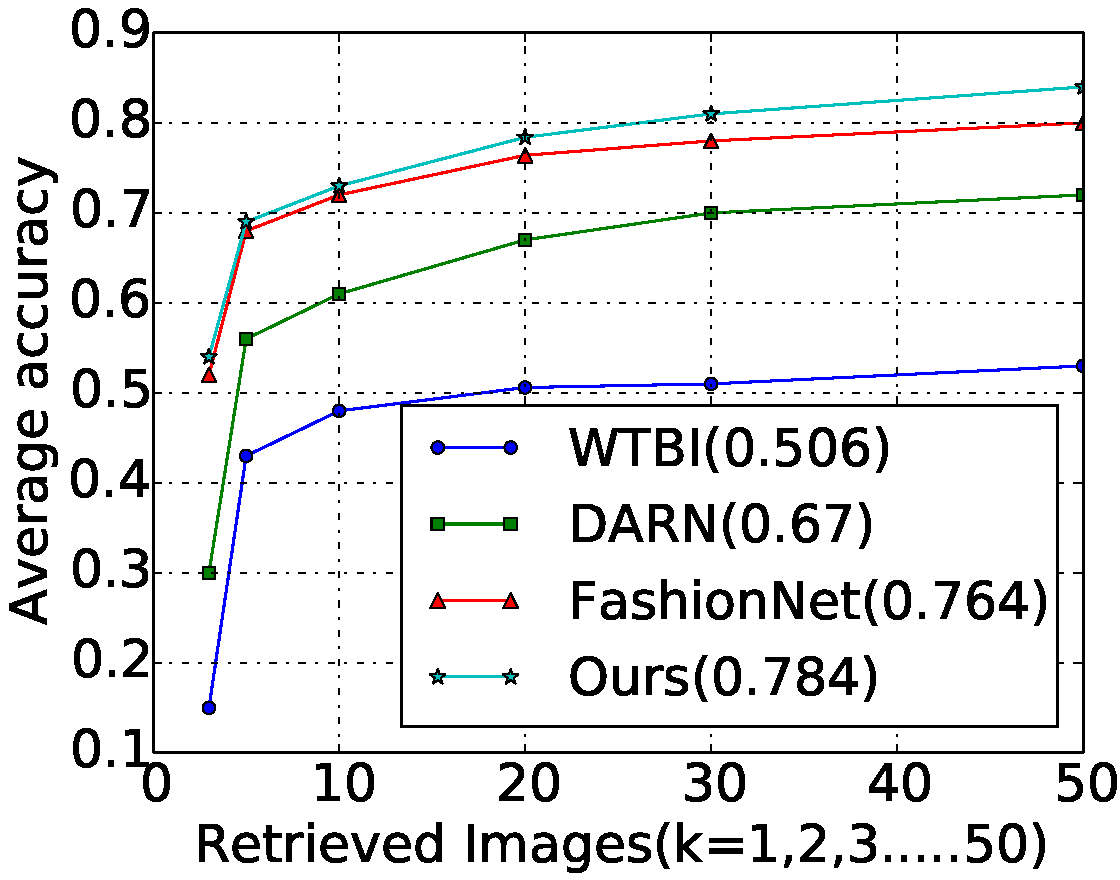
\includegraphics[width=0.48\linewidth]{images/Inshop} }}
    \subfloat[Consumer-to-shop retrieval]{{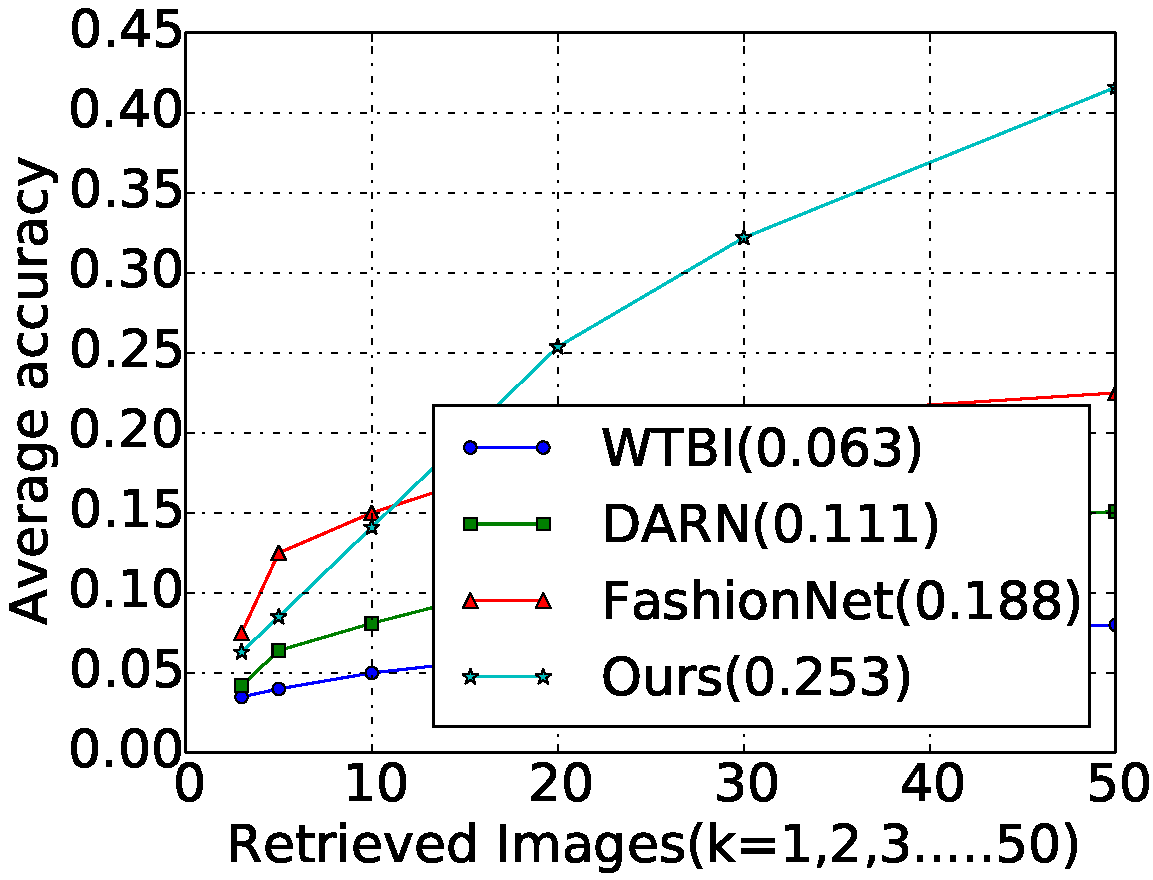
\includegraphics[width=0.48\linewidth]{images/Consumer2shop} }}
  \end{figure}
\end{center}
Retrieval results for In-shop and Consumer-to-shop retrieval tasks on DeepFashion dataset \cite{LiuCVPR2016}.
\end{frame}

\begin{frame}{Results}
\vspace{-1cm}
\begin{center}
  \begin{figure}
    \centering
    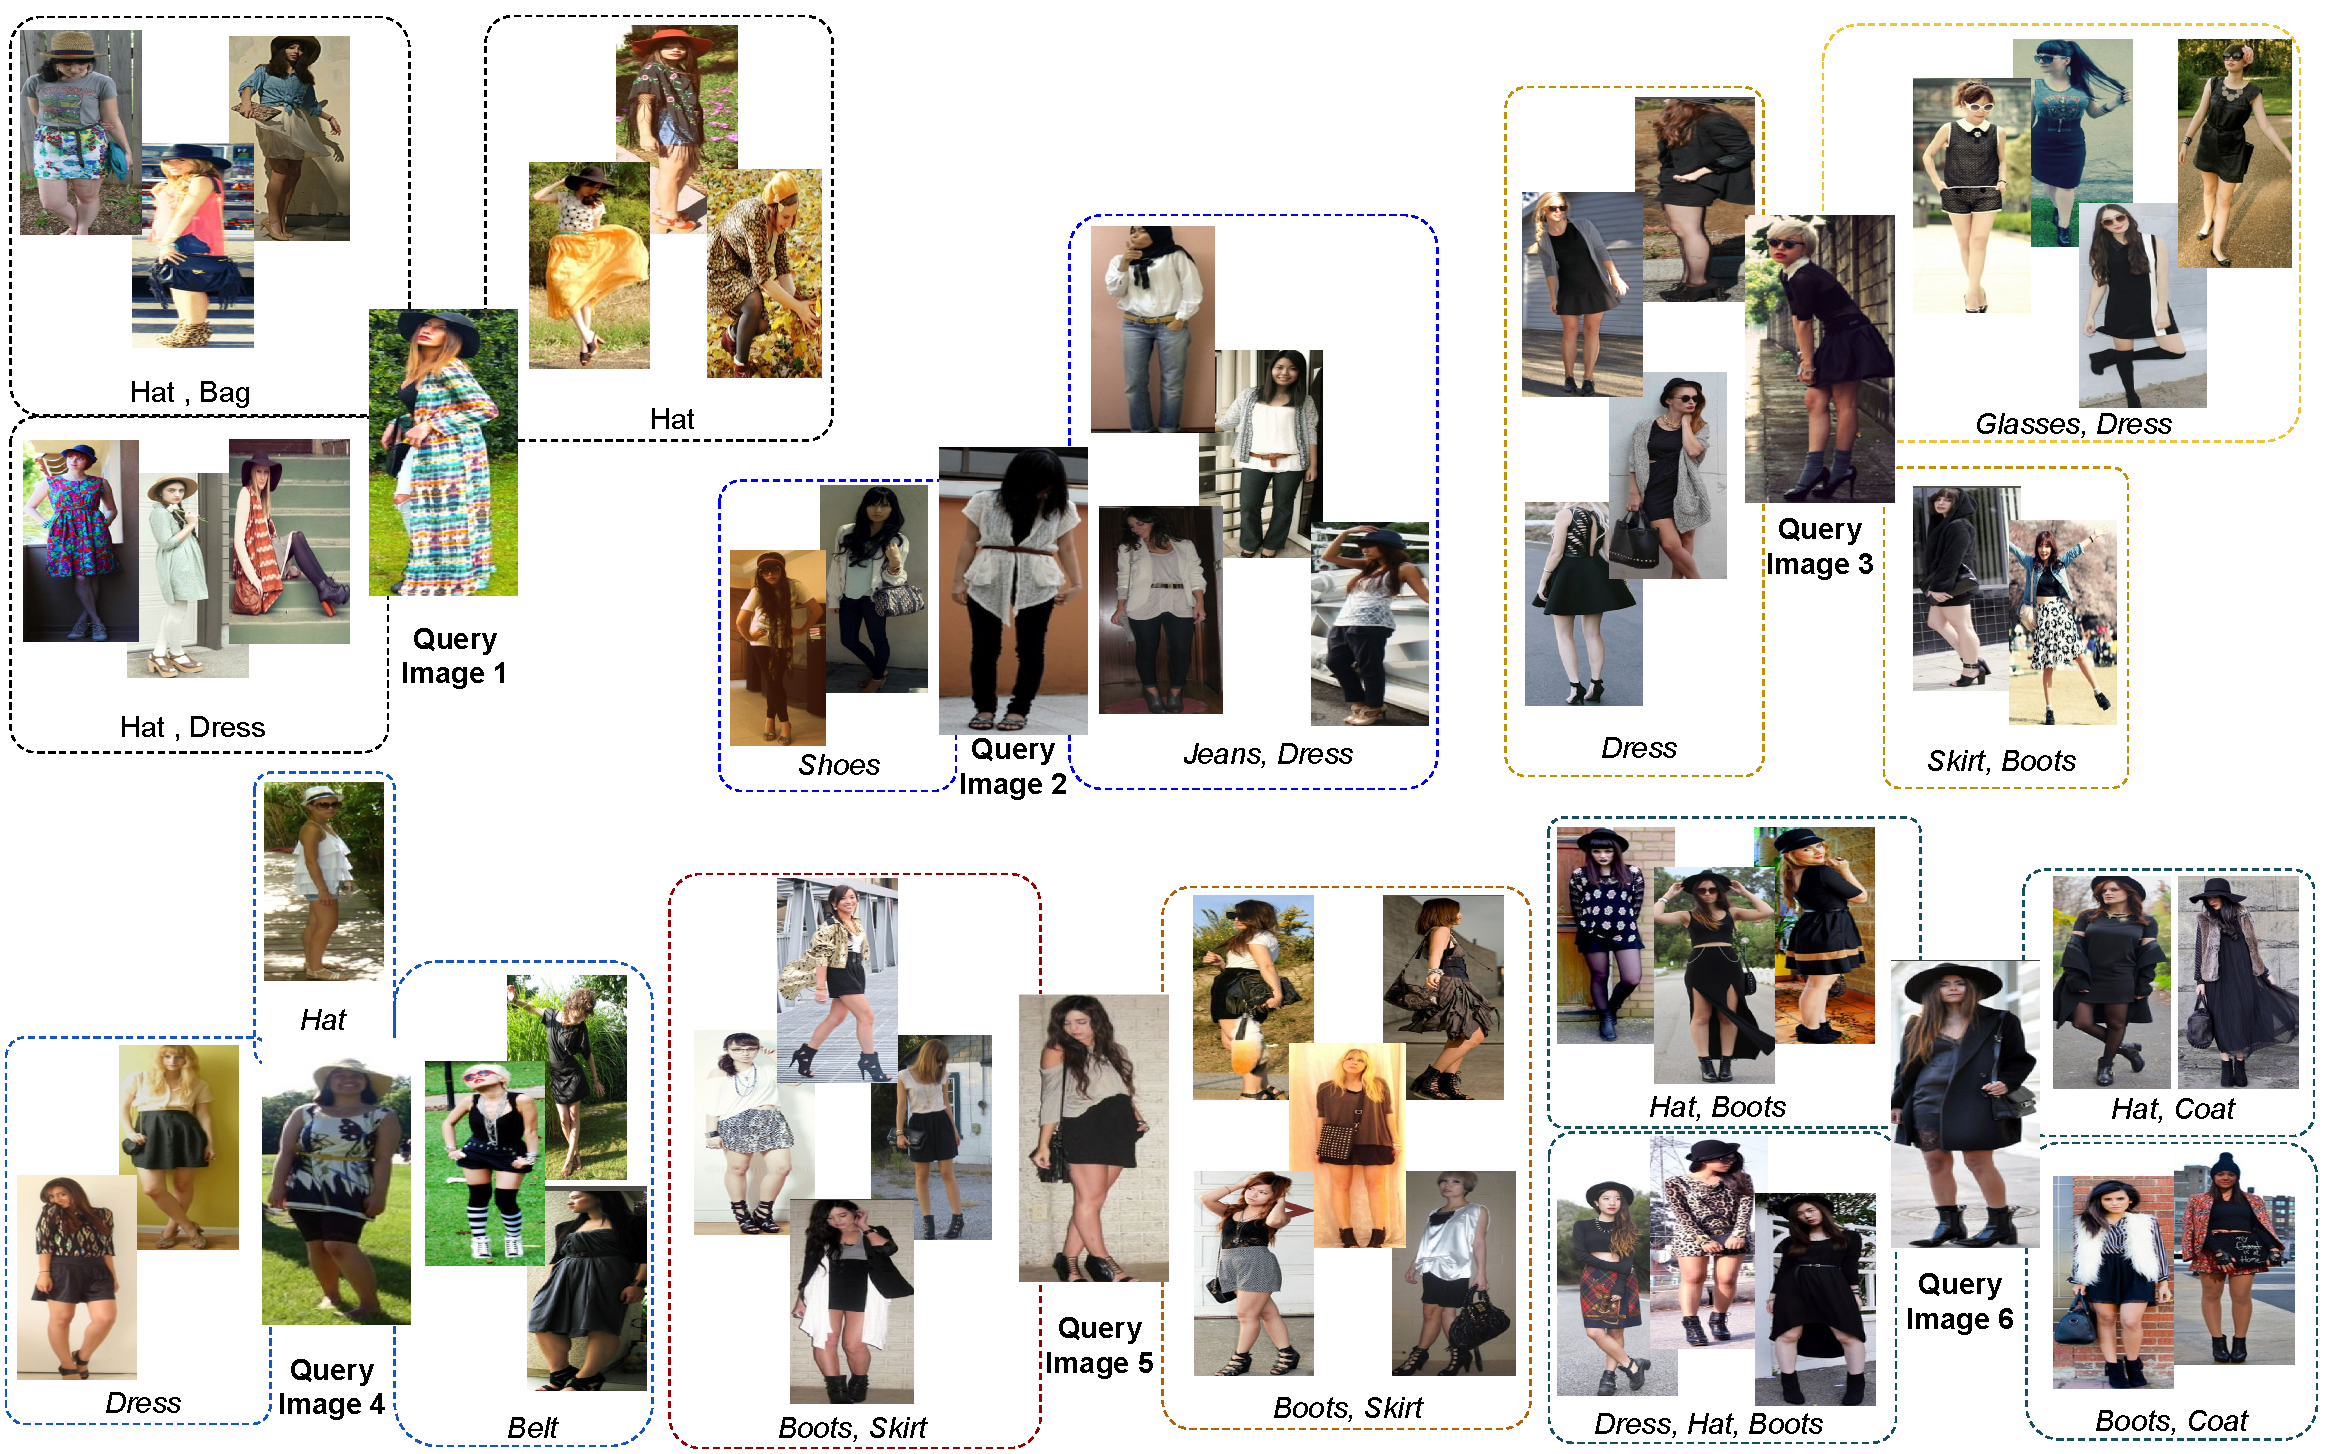
\includegraphics[width=0.8\linewidth]{images/staqu_results}
  \end{figure}
\end{center}
Semantically similar results for some of the query images from Fashion144k dataset \cite{SimoSerraCVPR2016} using our method.
\end{frame}

\begin{frame}{Conclusion}
  \begin{itemize}
    \item Using clothing parts for recommendation gives much variability in the recommendation results.
    \item Attention can be used to learn discriminative features from weak labels.
    \item Texture cues are important for learning different parts.
  \end{itemize}
\end{frame}

\begin{frame}{References}
  \bibliographystyle{IEEEbib}
    \tiny\bibliography{refs}
\end{frame}

\begin{frame}
\huge{Thank you}\\
\huge{Questions?}\\
\end{frame}

\end{document}